% main.tex: Paper 1, critical systematic review for ACM Computing Surveys.
% Class: acmart v2.20 (2026/08/16), installed in MiKTeX; same version as the pinned copy in
% paper/style/acm/minimal-csur/ (see research/review/dossier/csur.md Part A).
% Page counting uses acmsmall (6.75 x 10 in). For the review submission switch to
% \documentclass[manuscript,review]{acmart} (csur.md section 2); its page count is not the CSUR count.
% Build: latexmk -pdf main.tex   (bibliography: ACM-Reference-Format.bst, copied from paper/style/acm/minimal-csur)
\documentclass[acmsmall]{acmart}

\AtBeginDocument{\providecommand\BibTeX{{Bib\TeX}}}
\citestyle{acmnumeric}

\acmJournal{CSUR}
% Filled by ACM at production:
\acmVolume{1}\acmNumber{1}\acmArticle{1}\acmMonth{1}\acmYear{2027}

% ---- drafting aids (removed at submission) ----
% \todo marks a missing fact, a pending audit or an author query ([AUTHOR: ...] convention).
\newcommand{\todo}[1]{{\color{red}\textbf{[TODO: #1]}}}
% \aud tags a number that comes from census-result-v2.md and awaits the gate audit.
\newcommand{\aud}{\textsuperscript{\color{red}\scriptsize audit}}

\begin{document}

\title[Diffusion Language Models and Unified Multimodal Generation]{Diffusion Language Models and Unified Multimodal Generation: A Critical Systematic Review of Discrete and Continuous Approaches}
% Working title, decision D0007 (research/ledgers/decisions.jsonl). Not "and Meta-Analysis": the pooling threshold is not met.

\author{Shlok Kumar Goenka}
\affiliation{%
  \institution{Vellore Institute of Technology}
  \city{Vellore}
  \state{Tamil Nadu}
  \country{India}}
\email{shlok.goenka2023@vitstudent.ac.in}
% [AUTHOR: second author is the professor; name, school and e-mail are not recorded in research/ or research/review/dossier/]
\author{[AUTHOR: name of the professor]}
\affiliation{%
  \institution{Vellore Institute of Technology}
  \city{Vellore}
  \state{Tamil Nadu}
  \country{India}}
% TODO (author query): ORCIDs for both authors and the single corresponding author (ACM requires them at submission).

\begin{abstract}
% Rule: at most 100 words, no first person, no citations (csur.md section 2). Written last; numbers need the gate audit.
\todo{abstract is a placeholder, written last. Draft: Diffusion language models and unified multimodal diffusion models are reviewed under PRISMA 2020 from \todo{N} included studies. We place 47 models in one design space, count how many headline results state and hold fixed their value rule in a random sample of the corpus, organise sampler error as a budget with a single value term, and state open problems with the evidence each needs. In a random sample, 147 of 153 papers with a generated-sample or samples-only headline use a non-plain value rule or do not state one \todo{audit}.}
\end{abstract}

\ccsdesc{General and reference~Surveys and overviews}
\ccsdesc{Computing methodologies~Natural language generation}
\ccsdesc{Computing methodologies~Machine learning}
% TODO: generate the CCSXML block with the ACM indexing tool (csur.md section 2); concept ids are not copied from memory.
\keywords{diffusion language models, masked diffusion, discrete diffusion, unified multimodal models, decoding, systematic review}

\maketitle

% Section 1. Introduction. Carries all contributions (C1-C4) and the not-claimed list.
% Evidence map: paper/review/OUTLINE.md section 2, "1 Introduction".
\section{Introduction}
\label{sec:intro}

A diffusion language model (DLM) generates text by repeatedly predicting many positions in parallel and committing a subset of them, rather than emitting one token at a time from left to right. \citet{arXiv:2107.03006} introduced diffusion on categorical state spaces; later work specialised it to the masked, or absorbing-state, case~\cite{arXiv:2310.16834,arXiv:2406.07524,arXiv:2406.04329,arXiv:2406.03736}, developed a parallel line that diffuses continuous embeddings~\cite{arXiv:2205.14217}, and trained such models at the scale of autoregressive language models~\cite{arXiv:2502.09992}. The same machinery now underlies unified models that understand and generate more than one modality with a single network~\cite{arXiv:2503.20853,arXiv:2505.15809,arXiv:2408.12528}. The literature is growing quickly: of the 540 records with an arXiv identifier in the curated list that seeds our corpus, 243 first appeared in 2026 and only 19 in 2022 or earlier.

This article reviews that literature systematically. From 79,963 identified records, 615 studies were included; a stratified random sample of them was extracted in full and appraised for quality. Beyond describing methods, the review organises the field around five design choices that every generator makes, asks how well the published evidence supports the field's main claims, and records how the headline results of a random sample of papers were decoded. The rest of this section explains why such a review is needed (Section~\ref{sec:intro-why}), positions it against earlier surveys (Section~\ref{sec:intro-related}), and states the research questions, the contributions and the organisation of the article.

\subsection{Decoding choices and the comparability of reported results}
\label{sec:intro-why}


Comparing results across this literature is hard for a reason particular to how these models are used: a DLM has no canonical way to sample from it. The number a paper reports depends on how many positions are committed per step, which positions, and how the committed values are chosen (the \emph{value rule}): drawn at temperature one, sharpened, truncated, guided, or selected from several candidates. Papers differ in all of these and often do not say which they used. Recent evaluation studies have begun to document the consequence. One reports that the ranking of parallel-decoding methods depends on the prompt template~\cite{arXiv:2606.29228}; another examines how efficiency is evaluated across papers~\cite{arXiv:2510.18480}; a technical note discusses benchmark choice and the relation between generative perplexity and entropy~\cite{arXiv:2604.02718}. % src: research/review/survey-landscape.md sections 1c and 2 (E1: abstracts read, not full texts); research/ledgers/papers.jsonl P0079, P0078, P0023, P0113

This review asks how well the published evidence supports the field's claims, and it organises the design choices of these models so that the question can be asked precisely. Search and selection follow PRISMA~2020~\cite{page2021prisma}, and each body of evidence is judged rather than only described.

\subsection{Prior surveys of diffusion language and unified multimodal models}
\label{sec:intro-related}

Two surveys are closest to ours in scope. The survey of \citet{arXiv:2508.10875} (version~3, over 220 references) covers continuous, discrete and hybrid models, training, inference, multimodal models and applications. Its performance study compares DLMs with autoregressive models on eight benchmarks using numbers that are, in its words, primarily taken from the original publications. % src: research/review/survey-landscape.md section 1a (row 2508.10875 v3: refs 228; Sec VI Performance Study)
\citet{arXiv:2506.13759} (version~5, 175 references) cover the discrete case with catalogue tables. % src: research/review/survey-landscape.md section 1a (row 2506.13759 v5: refs 175)
Other surveys address unified multimodal models~\cite{arXiv:2505.02567,arXiv:2409.14993,arXiv:2605.25343}, parallel text generation~\cite{arXiv:2508.08712}, inference efficiency~\cite{arXiv:2607.12829}, edge deployment~\cite{arXiv:2609.04778}, alternatives to next-token prediction~\cite{arXiv:2509.24435} and earlier diffusion-for-text work~\cite{arXiv:2303.06574}.

In a keyword scan of the full texts of sixteen related surveys and tutorials, none states a search protocol with database strings, screening counts and a flow diagram. % src: research/review/survey-landscape.md claims block and section 1a. Reconciled 2026-10-21: the claim block's "14" predates two rows added to table 1a (arXiv:2512.05092, a tutorial, protocol "not applicable"; arXiv:2608.20743, protocol "none found"), so all 16 rows lack a stated search protocol.
One presents itself as a survey conducted through a systematic review and gives venues, years and inclusion criteria, but no search strings or counts~\cite{arXiv:2509.24435}; another gives inclusion criteria for one subsection~\cite{arXiv:2508.08712}. % src: survey-landscape.md section 1a (rows 2509.24435, 2508.08712)
None of them audits what the surveyed papers report: seeds, intervals, matched compute, or the sampling rule behind the headline number. % src: survey-landscape.md section 1a, columns "Audits reporting" (none found in any Tier-1 row)
Neither close survey places models in a design table whose columns are design choices. \citet{arXiv:2506.13759} give no comparison table, and the 36-model table of \citet{arXiv:2508.10875} has mostly metadata columns, of which only the diffusion type is a design choice. % src: research/review/dossier/competitor-anatomy.md section 3, verdict ii
The survey of \citet{arXiv:2508.10875} also states the independence of parallel predictions as a qualitative problem, without a decomposition. % src: competitor-anatomy.md section 3, verdicts iii and iv
We do not claim to be the first survey of this area; the contribution is a different kind of review: a documented search and selection, a design space tested on named models, a census of how results are decoded and reported, and an error budget used to classify methods.

\subsection{Research questions and evidence base}
\label{sec:intro-rq}

The protocol, which follows the guidelines of Kitchenham and Charters for systematic reviews in computing~\cite{kitchenham2007guidelines}, fixes six research questions, each answered from evidence in a dedicated subsection; RQ2 to RQ5 end with a verdict (well supported, weakly supported, mixed or untested). % src: research/review/protocol.md sections 1 and 7
\begin{description}
  \item[RQ1] Which formulations of diffusion language models and unified multimodal diffusion models exist, and what separates them (state space, forward process, objective, parameterisation, sampler)?
  \item[RQ2] How do these models compare with autoregressive models, and under which protocols were the comparisons made?
  \item[RQ3] What do training strategies contribute (pretraining recipe, instruction or reasoning fine-tuning, reinforcement-learning post-training, distillation)?
  \item[RQ4] How does inference trade quality against compute (denoising steps, unmasking order, remasking, caching, parallel decoding)?
  \item[RQ5] In unified multimodal models, what evidence supports, limits or contradicts understanding--generation synergy?
  \item[RQ6] How rigorous is the evidence base (reporting, reproducibility, statistics, agreement between a paper's claims and its own tables)?
\end{description}
% src for the six questions: research/review/protocol.md section 1 (wording shortened only in RQ5 by dropping "evidence used")

Not every question rests on every included study. RQ1 is answered from the screening fields of all 615 included studies, from the 47 models of the design-space table (Section~\ref{sec:design}) and from a stratified sample of the included studies extracted in full. RQ2 to RQ6 are answered from that sample (59 included studies, with 20 seed-corpus studies reported apart), with shares weighted to the size of each stratum and given with intervals (Section~\ref{sec:rq}). The census of Section~\ref{sec:census} reads a random sample of the seed corpus to code the value rule behind each headline number, and the seed-corpus stratum of the extraction sample is drawn from it. % src: sections/05-rq-evidence.tex; analysis/extraction/d0052/ (D0051, D0052, D0054, D0060)

Too few comparisons in the literature share a task, a metric and a compute budget for a meta-analysis, so the review reports counts and weighted shares with intervals rather than a pooled estimate.

\subsection{Contributions of this review}
\label{sec:intro-contrib}

The review makes four contributions and credits the work each builds on. Section~\ref{sec:practice} condenses them for practitioners as canonical models mapped onto the five choices, decoding defaults and a reporting checklist.

\paragraph{A design space in one notation, tested on 47 models.}
Every generator in scope is written as a choice of channel, reveal law, predictor, commitment policy and revision rule, with fourteen levers that change quality or cost (Sections~\ref{sec:notation} and~\ref{sec:design}). The notation builds on published unification results for the masked case~\cite{arXiv:2406.07524,arXiv:2406.04329,arXiv:2406.03736}; we do not claim them. Of the 47 models, 36 fit the notation fully and 11 fit it partly, and every model could be placed; the 11 partial fits mark the stated limits of the notation. % src: research/review/coverage/design-space-v1.csv (column "fits": yes 36, partly 11; counted by script 2026-10-15); design-space-v1.md claims block
The test is less demanding than the count suggests, because the vocabulary was written to be inclusive and 29 of the 47 rows were taken from earlier readings of primary sources rather than re-read for this table. % src: design-space-v1.md "competing_explanations" and "How to read the table" (M01 to M29 copied from the primers)

\paragraph{A census of value rules and reporting.}
In a random sample of 176 records drawn from the 1,106 that both screeners passed to full text and that have an arXiv identifier, 167 papers were eligible. For 153 of them the value rule behind the headline result can be coded (152 report a generated-sample metric and one shows samples only). Of those 153, 147 (96\%, 95\% interval 92 to 98) either decode the headline with a value rule other than plain sampling at temperature one, or do not state the rule. Of the 152 with a metric, 28 pair the headline with a diversity or entropy measure, and of the 55 that report the headline at two or more step settings, 20 state that the value rule was held fixed (Section~\ref{sec:census}). % src: research/review/coverage/census-result-v2.md ("Result", commit 8dd2af3); analysis/census/summary-random.log (final block)
That reported quality and fairness depend on the sampling or evaluation setting has been argued for other metrics and model families~\cite{arXiv:2606.29228,arXiv:2606.20536,arXiv:2607.24763}; the census quantifies the reporting gap for diffusion language models. % src: census-result-v2.md ("What can be said", credit sentence); decisions D0019, D0021

\paragraph{The error budget as a taxonomy.}
For any sampler, described by its commit kernel (the joint law of the positions it commits and the values it gives them; Section~\ref{sec:notation-process}), the divergence between data and sampler along a data path with the same position law splits into a factorisation term, a learning term and one signed value term $V$ that collects every departure of the committed values from the product of the predicted marginals (Section~\ref{sec:budget}). The two-term case $V=0$ is published~\cite{arXiv:2505.24857}; the three-term form is a corollary of the chain rule that we write out. Other pieces are published and we credit them: the majorisation argument for a one-token commit and the sample--select--resample correction~\cite{arXiv:2605.12522}; the distinction between sampling then choosing and choosing then sampling, and the closeness of noised MaskGIT~\cite{arXiv:2202.04200} to a tilted sampler~\cite{arXiv:2510.04525}; the split between confidence-based remasking and top-probability selection~\cite{arXiv:2609.34509}; and the best-of-$N$ KL and win-rate bounds~\cite{arXiv:2401.01879}. % src: research/review/framework-v2.md sections A and B; dossier/prior-art-selection.md
We treat $V$ as a bookkeeping device that locates where a sampler's value rule acts. It is not a quantity with a canonical size: the split depends on the data-path coupling and, for any ``selection'' share, on a reference policy. % src: framework-v2.md section B (paragraph beginning "The decomposition is not unique")

\paragraph{Open problems with the evidence each needs.}
Each open problem is stated with what is known now, the measurement that would settle it, and what would refute it (Section~\ref{sec:open}). They concern what a step sweep identifies and what it does not; whether a revision sampler's gain survives matching the value rule; whether cross-modal dependence in a unified model is concentrated in the early steps, and whether schedules that avoid committing dependent text and image positions together help; and a four-arm measurement on one frozen checkpoint that separates sample-then-filter selection from its resampled and tilted variants. % src: research/review/framework-v2.md sections C (P1, P3, P5) and D item 4

\subsection{What the review does not claim}
\label{sec:intro-notclaimed}

The notation, the census and the error budget serve the survey: they organise and evaluate the published work rather than propose new methods. We do not claim a selection error or a tilt cost as new error terms; we examined both and set them aside. % src: research/ledgers/decisions.jsonl D0011; research/review/framework-v2.md section A
We make no claim of a per-step impossibility result, of the size of the value term, the coupling term or the cross-modal dependence on a real model, or of the U-shaped dependence on the number of steps that appears in a toy model. % src: framework-v2.md section D "Not claimed"
We do not claim that the census sample is a sample of the whole field: it is a random sample of records that passed title-and-abstract screening and have an arXiv identifier. We do not claim that sampler effects on joint text--image consistency are new, or that the value rule carries that consistency; the single preregistered run of Section~\ref{sec:exp003} supports neither claim. % src: research/review/audits/2026-10-15-gate-EXP-003.md section 6 items 4 and 7; decision D0019

\subsection{Organisation of the article}
\label{sec:intro-guide}

\suppFigTree{} in the Supplement places the 47 models of the design space (Section~\ref{sec:design}) in a taxonomy by state space and model family, and gives an entry point to the literature: each leaf cites the model's paper. % src: research/review/coverage/design-space-v1.csv ("family"); scripts/fig_taxonomy.py


Section~\ref{sec:method} gives the review method, Section~\ref{sec:notation} the notation, Section~\ref{sec:design} the design space, Section~\ref{sec:rq} the evidence by research question, Section~\ref{sec:census} the census, Section~\ref{sec:budget} the error budget and Section~\ref{sec:practice} what the evidence means for practice. Section~\ref{sec:open} sets out the open problems, with a preregistered check on a frozen unified model (Section~\ref{sec:exp003}), and Section~\ref{sec:limits} the threats to validity. The full search strings, the PRISMA checklist, the codebooks and the row-level tables are in the Supplement.

% Section 2. Review method. Rewritten 2026-10-20 (session 0839c9f4) for the state after the search update, the
% subscription databases, full-text tranche T1, the re-check tranche R797 and the screening freeze D0051; the census
% subsections are kept from the 2026-10-15 draft. Every count has a % src comment; flow counts come from
% analysis/prisma/prisma-flow.json (script analysis/prisma/prisma_flow.py) unless stated.
\section{Review method}
\label{sec:method}

\paragraph{The method at a glance.} Three identification strands (a curated seed corpus, a search update over free sources and six subscription databases) fed one screening pipeline: two independent automated screeners per record, an adjudicator for disagreements, fixed written criteria, and verbatim quotes matched against each paper. Screening was frozen on 2026-10-20 with 615 included studies. RQ1 counts use fields recorded for all 615; RQ2 to RQ6 use a stratified random sample of 80 studies, extracted with a fixed form and appraised on nine quality items; a census of a random sample of seed records codes the value rule behind each headline result. The section ends with the departures from the protocol; the full list is in the Supplement (Section~S1), and Section~\ref{sec:limits} states what each does to the conclusions.

\subsection{Design, reporting standard and protocol status}
\label{sec:method-design}

The review is reported against PRISMA~2020~\cite{page2021prisma} (checklist in the supplement, Section~S1) and follows Kitchenham and Charters' procedure for systematic reviews in computing~\cite{kitchenham2007guidelines}. The protocol (research questions, eligibility, sources, selection, extraction, appraisal, synthesis) is archived with the data and code (version~0.1 of 2026-10-13). % src: research/review/protocol.md header line "DRAFT v0.1, 2026-10-13; not frozen"
It was \emph{not} frozen or registered before screening: the freeze rule asked for a git tag after sign-off, and none exists. % src: protocol.md "Freeze rule"; `git tag` returned no tags on 2026-10-15
Amendments are recorded in protocol section~10 and in a decision ledger with one row per decision (identifiers D0001 onwards, cited below); Section~\ref{sec:method-deviations} lists every departure. % src: protocol.md section 10; research/ledgers/decisions.jsonl

\subsection{Information sources and searches}
\label{sec:method-sources}

The search ran in three strands (Table~\ref{tab:sources}; Figure~\ref{fig:prisma}). The \emph{seed corpus} joined a curated list of diffusion language model papers with two logged arXiv searches of 2026-10-14. The \emph{search update} of 2026-10-15 ran revised strings on five free sources and snowballed citations from the seed; the strings were revised after the protocol's recall pilot failed, and the final strings kept seed recall at 525 of 540. The \emph{subscription strand} searched six databases on 2026-10-15 and 2026-10-16 through institutional access. Every query, date and hit count is logged; the strings, the recall checks and the export limits are in the Supplement (Section~S1).

\begin{table}[t]
\caption{Sources searched and records identified, before deduplication. Counts from the search log and the merge statistics; the full strings are in the supplement (Section~S1).}
\label{tab:sources}
\small
\begin{tabular}{@{}p{5.1cm}p{2.9cm}r@{}}
\toprule
Source & Date & Records \\
\midrule
\multicolumn{3}{@{}l}{\emph{Seed corpus}} \\
Awesome-DLMs list (commit 194aa6bd) & parsed 2026-10-13 & 572 \\ % src: prisma-flow.json seed.identified_awesome_dlms
arXiv API, strings S1 and S2 & 2026-10-14 & 1,331 \\ % src: prisma-flow.json seed.identified_arxiv_S1 1158 + S2 173
\multicolumn{3}{@{}l}{\emph{Search update (strings S1, S2, S1$'$, S2$'$)}} \\
Semantic Scholar bulk API & 2026-10-15 & 10,572 \\ % src: prisma-flow.json free.identified_databases_by_source
arXiv API & 2026-10-15 & 6,105 \\
OpenReview API & 2026-10-15 & 3,357 \\
OpenAlex & 2026-10-15 & 1,081 \\
ACL Anthology & 2026-10-15 & 355 \\
Citation searching, backward and forward & 2026-10-15 & 45,421 \\ % src: free.identified_citation_searching (19423 + 25998)
\multicolumn{3}{@{}l}{\emph{Subscription databases}} \\
Scopus & 2026-10-15 & 4,046 \\ % src: prisma-flow.json subscription.identified_by_database
SpringerLink & 2026-10-16 & 2,614 \\
Web of Science Core Collection & 2026-10-15 & 2,267 \\
IEEE Xplore & 2026-10-15 & 1,300 \\
ScienceDirect & 2026-10-16 & 613 \\
ACM Digital Library & 2026-10-15 & 329 \\
\midrule
Total identified & & 79,964 \\ % src: 1903 + 66891 + 11169 (fig01-prisma.log seed_id, upd_id; subscription.identified)
\bottomrule
\end{tabular}
\end{table}

\paragraph{Deduplication and automation filters.} Records were merged on shared identifiers and normalised titles, leaving 1,453 seed records, 19,328 new update records and 4,380 new subscription records. The final strings were then applied locally and excluded 17,486 update and 4,201 subscription records by automation; a validation of that filter crossed its preset reversal threshold, so a single-screener rescue pass read every filtered record with an abstract (Supplement, Section~S1).

\subsection{Eligibility}
\label{sec:method-eligibility}

A record is included if it satisfies all of the following. It proposes, analyses, evaluates or benchmarks (a) a diffusion model, in discrete or continuous state space, whose output includes natural-language text or code, or (b) a unified model, one model and not a pipeline, that both understands and generates across text and at least one other modality (image, video, audio or speech, or 3D) with a diffusion, masked-generative or discrete-flow component. It is a primary study with a method, theory or empirical result. Its full text is in English, and its first public version is dated 2021-01-01 or later. % src: protocol.md section 2 (I1 to I4) and section 10 (I1(b) amendment, decision D0020)
Exclusions carry one code: X0 no diffusion component, X1 non-text diffusion not covered by (b), X2 text only as conditioning, X3 secondary study, X4 no method, theory or result, X5 duplicate, X6 full text unavailable, X7 application of an unchanged model with no model-level finding, X8 outside the date window or not English. % src: screening/criteria-v1.6-screener.md; decision D0032
Full-text screening applied criteria v1.6, which fixes the order in which codes are tried and how a diffusion component is recognised; it was revised through five red-team audits before the first full-text decision. % src: decision D0032; research/review/audits/2026-10-16-redteam-criteria-v1.1.md to -v1.5.md

\subsection{Selection process and agreement}
\label{sec:method-screening}

\paragraph{Title and abstract.}
Two automated screeners (see the Declaration on the use of AI) read each record independently from fixed written criteria, blind to each other; a record passed to full text if either marked it include or unclear (decision D0030). % src: decision D0030; screening/v2/SCREENER-BRIEF.md
In the seed strand the two screeners agreed on pass against exclude for 1,333 of 1,453 records ($\kappa=0.728$)~\cite{cohen1960coefficient}. % src: tools/screening_agreement.py output (2026-10-15): "pass-to-full-text agree 0.917 kappa 0.728"; screener-B/run-log.jsonl
In the update and subscription strands they agreed with $\kappa=0.911$ (95\% bootstrap interval 0.892 to 0.929) on 1,953 records, and $\kappa=0.930$ (0.861 to 0.985) on the first 246 of 260 subscription records, the other 14 agreeing in every case. % src: analysis/screening/agreement-v2.log ("pass vs exclude raw 0.955 kappa 0.911 [0.892, 0.929]"); screening/v2/dual-subscription/agreement-sub.json (n 246, kappa 0.9302 [0.8614, 0.9852]), agreement-sub-02.json (10 of 10), agreement-sub-03.json (4 of 4)
1,243 seed records, 954 update records and 52 subscription records passed. % src: prisma-flow.json seed.ta_pass_either, free.ta_pass_D0030, subscription.ta_pass_D0030

\paragraph{Full text.}
Full texts were retrieved from open-access sources or through the institutional e-gateway, logged and hashed, converted to text with page markers, and checked against the record's title. % src: research/review/fulltext/fetch-log.jsonl; analysis/screening/ft-t1/t1-provenance.jsonl; tools/ft_title_check.py
Each batch of about ten records went to screener~A and screener~B in separate dispatch folders that held only the criteria, the batch's texts and an output file. Every decision had to cite verbatim evidence with its page; a script checked each quote against the text and returned an unmatched quote to its screener once. Disagreements, ``adjudicate'' rows and quotes still unmatched went to an adjudicator, who saw both rows. % src: criteria-v1.6.md section 4 items 1-5; tools/ft_dispatch.py; quote_check.py; analysis/screening/c-run-log.jsonl (route F line, 2026-10-16)
Each session's transcript was checked for reads outside its folder and for the model that produced every turn; a session that failed either check was discarded and rerun. % src: tools/ft_isolation_check.py; tools/ft_model_check.py; research/progress.md HANDOFF 18 (t1b081 B rerun)
Tranche T1 assessed the update and subscription passes: 885 reports, all decided, 608 included and 277 excluded (X0 77, X1 103, X2 85, X3 7, X4 4, X7 1); the adjudicator ruled on 116, and 3 of the exclusions are the records screener~B could not read (below). Before adjudication, A and B agreed on pass against exclude with $\kappa=0.894$ (0.859 to 0.927; $n=882$). % src: prisma-flow.json full_text_T1 (decided_incl_resolved 885, include_incl_resolved 608, exclude_incl_resolved 277, exclude_codes_incl_resolved, adjudicated_by_C 116, kappa 0.8939 [0.8589, 0.9268]); analysis/screening/agreement-ft-t1.json; decisions D0058, D0059
208 reports were not retrieved (Figure~\ref{fig:prisma}). % src: fig01-prisma.log t1_not_retrieved
For three biology papers and, later, one more, screener~B's sessions failed and their rows were discarded. For these four records the first author confirmed screener~A's reading (three exclusions X1 in T1, one X2 in R797); they have no independent second screening and are left out of every agreement statistic (decisions D0041, D0046, D0056, D0058). % src: decisions D0041, D0046, D0056, D0058; analysis/screening/b-unavailable-resolved.jsonl; prisma-flow.json full_text_T1.resolved_B_unavailable_D0058, full_text_R797.resolved_B_unavailable_D0058

\paragraph{Re-check of title and abstract exclusions.}
Because most title-and-abstract exclusions in the update rested on one model, 797 exclusions were flagged by preset rules as possible errors, a random 100 of them were screened at full text, together with 32 further records found by a keyword query. The preset rule sent all 797 to full text if any sampled record was included; 4 of the 82 sampled records screened were included, so the rule fired. % src: criteria-v1.6.md section 5.1-5.3; analysis/screening/ta-recheck-k.json (K 4: M03416, M10984, R0963, R1202; included 4, excluded 78, not_in_T1 18)
The remaining 715 formed tranche R797, screened as T1 until the freeze: 285 reports assessed and decided, 7 included and 278 excluded; agreement before adjudication was $\kappa=0.602$ (0.362 to 0.793) with raw agreement 0.961 and Gwet's AC1 0.957, the low $\kappa$ reflecting how few records passed. % src: prisma-flow.json full_text_R797; analysis/screening/agreement-ft-r797.json (n 284)

\paragraph{Human validation.}
The protocol asks a human author to screen a random 15\% of each full-text tranche blind and requires each model screener to reach $\kappa\ge0.70$ against that author. For T1 two of the authors read the 108-record sample without recording per-record decisions (decision D0034; authors' statement of 2026-10-20); the R797 sample of 108 was drawn before any download and was not screened before the freeze. After the analysis the first author checked three blind random samples instead, validated as described in the Declaration on the use of AI (decisions D0065, D0066). On 40 T1 records (20 included and 20 excluded by the models) the author and the final decision agree on 21 of the 30 both decided ($\kappa=0.41$, 95\% interval 0.09 to 0.71; 10 unclear; the exclusion code matches on all 11 joint exclusions), below the protocol's 0.70 and on fewer than its 100 records. On 12 extraction records the study-level flags agree in 31 of 34 pairs ($\kappa=0.82$), and on 24 census papers the value-rule class agrees for 21 ($\kappa=0.79$; Supplement~S9). Every other screening statistic above is agreement between two models. % src: decisions D0034, D0035, D0048, D0065, D0066; screening/human-validation-t1/sample-manifest.json; human-validation-r797/sample-manifest.json; analysis/screening/human-check-screening-agreement.json; analysis/extraction/d0052/human-check-agreement.json; analysis/census/human-check-census-agreement.json


\begin{figure}[p]
\centering
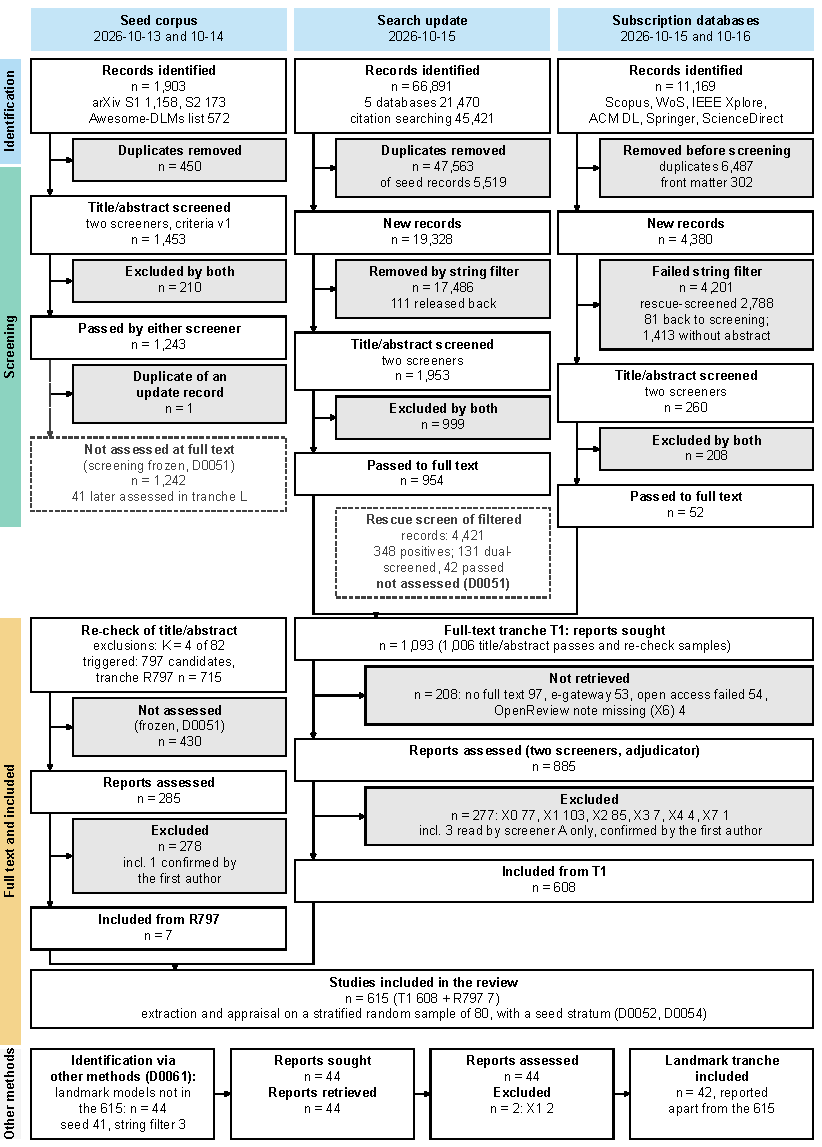
\includegraphics[width=\linewidth]{figures/fig01-prisma.pdf} % src: paper/review/scripts/fig01_prisma.py; every count read from analysis/prisma/prisma-flow.json, sums asserted, log figures/fig01-prisma.log
\caption{PRISMA 2020 flow. Three identification strands are screened separately and meet at full text. Grey boxes are records removed or excluded; dashed boxes are sets identified but not assessed at full text when screening was frozen (decision D0051). ``Awaiting second screener'' marks records that screener~B could not read and that the first author screens. X0 to X7 are exclusion codes (Section~\ref{sec:method-eligibility}). The bottom row is the landmark tranche, identified by other methods after the freeze (decision D0061).}
\label{fig:prisma}
\Description{A flow diagram in three columns. The seed corpus (1,903 records from a curated list and two arXiv searches) is deduplicated to 1,453 and screened by title and abstract; 1,243 pass, and 1,242 of these are not assessed at full text when screening was frozen (41 of them are assessed later in the landmark tranche). The search update identifies 66,891 records, of which 19,328 are new; a string filter removes 17,486; 1,953 are screened and 954 pass. The subscription databases identify 11,169 records, 4,380 new; 260 are screened and 52 pass. The update and subscription passes form full-text tranche T1: 1,093 reports sought, 208 not retrieved, 885 assessed, 277 excluded and 608 included. A re-check of title-and-abstract exclusions found 4 inclusions among 82 sampled records, which triggered tranche R797 of 715 records; 285 were assessed before the freeze and 7 included. In total 615 studies are included. A bottom row shows a landmark tranche identified by other methods: 44 papers of design-space models not in the 615, all retrieved and assessed, 42 included and 2 excluded, reported apart from the 615.}
\end{figure}

\subsection{Screening freeze}
\label{sec:method-freeze}

On 2026-10-20 the authors stopped screening to finish the review with the resources available (decision D0051). Three sets were identified but not screened at full text: the 1,242 seed records that passed title and abstract, the 430 R797 records not yet reached, and the 348 positives of the update's rescue pass (131 of them dual-screened, 42 passing). % src: decision D0051; prisma-flow.json not_screened_D0051 (seed_tranche_S1243_D0037.frame 1242, R797_remainder 430, free_source_rescue_positives_D0036)
The included set is therefore 615 studies (608 from T1 and 7 from R797): 596 from the search update, 13 from the subscription databases and 6 seed records that reached full text through the re-check of title-and-abstract exclusions. The seed records that passed title and abstract, which include widely used models such as LLaDA, MDLM, Dream and MMaDA, are therefore outside the screened set. To keep that strand in the evidence, the extraction sample adds a random seed stratum drawn from the census sample, whose full-text eligibility was judged by the census coders (Section~\ref{sec:method-extraction}; decision D0054). Section~\ref{sec:limits} discusses what the freeze does to each research question. % src: analysis/rq1/rq1-counts.json (n 615, by_tranche); rq1-includes.jsonl id prefixes M 596, U 13, R 6; research/progress.md HANDOFF 27 (R0128, R0205, R0246, R0350 in S1243); decision D0054
\paragraph{Landmark tranche.} After the freeze, the papers of the 44 design-space models (Section~\ref{sec:design}) that are not among the 615 were screened as a targeted tranche, identified by other methods (decision D0061): 41 unscreened seed records and 3 snowball records that the string filter had removed. All 44 full texts were retrieved and screened under criteria v1.6 by the same two screeners, who agreed on every include or exclude decision: 42 were included and 2 excluded (X1). A seeded random order of the 42 was fixed before extraction, and the first 16 were extracted with the same form and procedure as the sample until the compute budget was spent (decision D0063). The tranche is reported in its own column and changes neither the 615 nor any estimate for them. % src: analysis/screening/landmark/landmark-frame-summary.json (tranche_L 44; S1243 41, other 3); analysis/prisma/prisma-flow.json landmark_tranche_D0061 (identified 44, reports_retrieved 44, assessed 44, include 42, exclude 2, exclude_codes X1 2, agreement_A_B 44, adjudicated_by_C 0); analysis/extraction/lmk/extraction-order.json (seed 20261024, N 42); rq-results.json D0060 landmark_meta n_extracted 16; decisions D0061, D0063

\subsection{Data extraction and quality appraisal}
\label{sec:method-extraction}

\paragraph{All included studies (RQ1).}
For all 615 included studies the counts for RQ1 come from fields the screeners recorded at full text: the eligibility basis (I1(a), I1(b) or both), the modality, whether text is produced, the research questions the study bears on, and the year. Where the two screeners recorded different values the record is counted as split. % src: analysis/rq1/rq1_counts.py docstring; rq1-counts.json
\paragraph{Stratified sample (RQ2 to RQ6).} Evidence for RQ2 to RQ5 and the quality appraisal (RQ6) come from a stratified random sample of 80 studies (decisions D0051, D0052, D0054). Three strata cover the included studies: unified multimodal studies, and language-only studies split at the median text length into shorter and longer ones (52, 267 and 265 studies after later field resolutions; 59 sampled). A fourth stratum of 20 seed-corpus studies, drawn from those the census found eligible, is reported apart, as is the landmark tranche (decisions D0060, D0063). Shares are weighted to the stratum sizes, with 95\% bootstrap intervals; the estimator was chosen after extraction. The form (153 fields) records each paper's own comparisons as matched groups with their arms, metric, direction and budget, and nine appraisal items, QA1 to QA9: code, weights or data, evaluation protocol, run-to-run variation, uncertainty for the main comparison, baselines at matched or reported budget, an ablation of the credited component, claims that agree with the paper's own tables, and stated limitations. One automated extractor read each study and cited a page for every value; a validator checked every value against the text; a second extractor read 8 studies, and an adjudicator settled their differences from the full text. The two extractors agree on the values (616 of 616) and metric directions (75 of 76) of the contrast units both found and on most appraisal scores and study-level flags, but on only 5 of 8 direction flags, and they cut the same tables into comparison groups very differently (36 of 245 groups found by both, F1 0.29). Section~\ref{sec:rq} therefore draws no unit totals and makes its statements about studies. Twenty-seven records kept an entry the validator rejected; Supplement~S6 repeats the estimates without them. The full procedure is in the Supplement (Section~S4).

\paragraph{Synthesis.}
RQ2 to RQ5 are answered with a verdict (well supported, mixed, weakly supported or untested; protocol section~7) under thresholds stated in Section~\ref{sec:rq}. RQ1 and RQ6 are described. The abstract claim types (CT1 to CT6) are taken from the earlier claim-evaluability rubric and reported descriptively, because the synergy type did not reach reliability there. No meta-analytic pooling was attempted: the protocol's threshold of comparable contrasts on the same task, metric and budget is not met. % src: protocol.md section 7; research/review/feasibility/stage2/summary-*.md

\subsection{Census: sampling, coding and adjudication}
\label{sec:census-method}

The census of Section~\ref{sec:census} predates the search update and samples the seed corpus only; its eligibility judgements used the protocol's rules as amended on 2026-10-15 (decision D0020), not criteria v1.6. The pool is the 1,106 seed records that both title-and-abstract screeners passed and that have an arXiv identifier, put in a random order (seed 20261015) before coding; ranks 1 to 176 were coded, of which 4 have no full text, 5 are ineligible and 167 eligible. Two automated coders, blind to each other, coded the headline result, the value rule behind it (field F2) and four reporting fields; agreement was computed under codebook v1.1 before reconciliation, and adjudicators applied codebook v1.2, written afterwards. One possible leak of one coder's labels into the other's workspace is reported. The full procedure, with the stopping rule, codebook versions, adjudication counts and the incident, is in the supplement (Section~S3). % src: census-result-v2.md ("Sample", "Process", "Limits"); tools/census_sample.py (SEED 20261015); coverage/census-codebook-v1.md, -v1.1.md, -v1.2.md; decisions D0015, D0019, D0020, D0021

\subsection{Departures from the protocol}
\label{sec:method-deviations}

Twelve departures from the protocol are listed with their decision numbers in the Supplement (Section~S1). They fall into three groups. \emph{Protocol status:} the protocol was not registered before screening; the search strings were revised after a failed recall pilot; and the verdict definitions and thresholds, the estimator and the primary population were fixed after the results were known (Section~\ref{sec:rq} reports how far the verdicts depend on them). \emph{Selection:} screening was frozen before three identified sets were assessed, among them the seed corpus with the most-cited models (Section~\ref{sec:method-freeze}); the planned human validation was replaced by later author checks (Section~\ref{sec:method-screening}); and a few records were settled by the first author confirming an automated reading. \emph{Extraction and synthesis:} extraction covers a stratified sample of 80 studies by one extractor, with a second on 8; a claim-evaluability extension was suspended; the census codebook was amended after coding; the appraisal was run on the sample only; a landmark tranche was screened after the freeze and reported apart; and the comparability table, dose--response curves and appraisal by year and venue that the protocol promised are not given.


% Section 3. A unified notation. STUB (carries C1 and C3). Plan: OUTLINE.md sections 1 and 2, "3 A unified notation".
\section{A unified notation}
\label{sec:notation}

\todo{stub: write after the design-space table is frozen; at most 8 numbered equations, one symbol table, two short algorithms}

Plan.
\begin{itemize}
  \item Generation as a commitment process: a sequence $x$ drawn from $q$, a state $s_n=(z_n,m_n)$ of partially revealed or noised sequence and optional memory, and at each step a commit kernel with a position law and a value law. % src: research/review/framework-v1.md section 1; framework-v2.md section B
  \item The five choices C1 channel, C2 reveal law, C3 predictor, C4 commitment policy (position rule, value rule, joint draw), C5 revision, with the instances of each (erasure, symmetric, mixture and Gaussian channels; prefix, any-order and block reveal laws; marginal, ratio and embedding predictors; confidence, planner and joint-draw policies; remasking and output-level revision). % src: framework-v1.md section 1 table; dossier/primer-foundations.md section 0.1 and 2; primer-gaussian.md sections 1--3; primer-multimodal.md sections 1--3
  \item Unification claims with their restrictions: for the erasure channel the continuous-time bound is a weighted masked cross-entropy and equals the any-order autoregressive objective, so objectives coincide but model classes and samplers do not; the symmetric channel loses the time-free parameterisation; the Gaussian-to-uniform-state map of Duo holds per position and per time, not for trajectories. % src: framework-v1.md section 1 "Unification claims"; primer-foundations.md section 3 (verdicts); primer-gaussian.md Q5
  \item Derived quantities: parallelism $k_n=|A_n|$ and compute reuse. Symbol table (Table 3 in OUTLINE.md). Fig.~2 formalism diagram. Alg.~1 training objective in this notation; Alg.~2 generic commit-kernel sampler.
  \item Credit: every unification result is cited to its source; the notation is ours, the results are not.
\end{itemize}

% Section 4. Design space tested on 47 models (C1). STUB. Plan: OUTLINE.md "4 Design space on 47 models".
\section{The design space, tested on 47 models}
\label{sec:design}

\todo{stub: this section answers RQ1 for the 47 models of the table; it does not yet answer RQ1 for all included studies}

Plan.
\begin{itemize}
  \item The test: place each of 47 models in C1--C5 and in fourteen lever rows (L1--L14) using only the cell values the notation already names; ``fits'' means every choice is expressible and the factorisation identity applies as written, ``partly'' means a new value or an exception is needed. Result: 36 fit, 11 partly, none unplaceable. % src: research/review/coverage/design-space-v1.csv column "fits" (36 yes, 11 partly, counted by script 2026-10-15); design-space-v1.md section 0
  \item Selection of the 47: family balance (unified multimodal 15, Gaussian or embedding 7, absorbing 6, sampler-only 5, and others), rows M01--M29 copied from primer readings, M30--M47 read at section level; dropped candidates and why. % src: design-space-v1.md section 2
  \item The 11 partial fits define the stated limits of the notation: length-changing edit channels, stochastic memory, graded evidence at uncommitted positions, joint-over-set predictors, sequence-level selection. % src: design-space-v1.md section 3 (a) misfit list; claims block
  \item What the test could and could not fail: the vocabulary is inclusive, so a stricter test gives a lower fit rate; evidence level E2 at confidence 0.6 for the counts; no code (E3) inspected. % src: design-space-v1.md "competing_explanations", "coverage"
  \item Table: condensed 47-row table (long form in the supplement). Fig.: master taxonomy tree with citations at the leaves. Comparison with the two existing surveys' taxonomies. % src: dossier/competitor-anatomy.md sections 1--3
  \item Per-modality notes for unified models: guidance, per-modality weights and schedules, continuous image channels in hybrids and output-level revision are four additions, not ``no new machinery''. % src: framework-v1.md section 3 last paragraph
\end{itemize}

% Section 5. Evidence by research question. STUB. Needs gate R2 (full extraction and appraisal) before any verdict.
\section{What the evidence shows, by research question}
\label{sec:rq}

\todo{stub: no verdict may be written from the stage-two samples; needs the full extraction and the quality appraisal (QA1--QA9) of every included study}

Plan, one subsection per question, each ending with a verdict (well supported, mixed, weakly supported, untested) and the counts behind it.
\begin{itemize}
  \item RQ2, diffusion against autoregressive models: protocol-comparability table; pooled only where task, metric and budget match. No contrast table exists yet (stage two recorded none). % src: research/review/protocol.md section 1; feasibility/stage2/summary-steps.md (RQ2-vs-AR row: 0)
  \item RQ3, training strategies: within-paper ablations; the sampled strata have candidate rows but almost none with an interval. % src: feasibility/stage2/summary-steps.md and summary-remask-synergy.md (RQ3-training rows)
  \item RQ4, quality against compute: dose-response of step sweeps; non-monotone sweeps exist (quality peaks at 32 steps in two papers), so any interpolation rule must say what it does there; the census supplies the reporting side (Section~\ref{sec:census}). % src: feasibility/stage2/summary-steps.md ("Quality is not monotone in steps")
  \item RQ5, synergy: claims against the ablation that supports them. Of 8 unified-model papers in the sampled synergy stratum, 3 contain a real task-removal or shared-versus-decoupled contrast, direction mixed, no interval. Prior statements that synergy is conditional~\cite{arXiv:2609.01607,arXiv:2607.04423} and a benchmark reporting it largely absent~\cite{arXiv:2509.24897} are credited. % src: feasibility/stage2/summary-remask-synergy.md ("Synergy"); survey-landscape.md section 2 (CA)
  \item RQ6, rigour: quality appraisal table (supplement) and distributions by year and venue type; 92\% of rule-poolable contrasts in the stage-two sample report no variance. % src: summary-remask-synergy.md; protocol.md section 6
  \item Statement of the pooling decision: threshold of protocol section 7 not met for remasking and synergy, borderline for steps. % src: research/progress.md (2026-10-14 results); feasibility/stage2/summary-*.md
\end{itemize}

% Section 6. Census of value rules and reporting (contribution C2).
% Source of every number: research/review/coverage/census-result-v2.md at commit 8dd2af3 (corrected after the
% gate audit, decision D0021) and the logs it names. All numbers in this section are \aud until the
% audit corrections are re-verified by the gate-auditor.
\section{A census of value rules and reporting}
\label{sec:census}

\todo{audit: every number in this section comes from census-result-v2.md at commit 8dd2af3 (audit verdict PASS WITH CORRECTIONS, corrections applied); the gate-auditor must re-verify the corrected file before submission}

\subsection{Question and unit}
\label{sec:census-question}

The reported quality of a diffusion language model depends on how the committed values are chosen at each step (Section~\ref{sec:budget}). The census asks, for the headline result of each paper, whether a reader can tell which value rule produced it, whether that rule departs from plain sampling at temperature one, whether the diversity cost of the headline setting is shown, and whether a step sweep holds the rule fixed. It is a count of what the papers say. It does not measure how much any rule changed any number. The sample, fields, codebooks, coders and adjudication are described in Section~\ref{sec:census-method}.

\subsection{Agreement between the two coders}
\label{sec:census-agreement}

Table~\ref{tab:census-agree} gives agreement before any reconciliation, under codebook v1.1, on the 172 ranks that have a full text.% src: analysis/census/agreement-random.log; census-result-v2.md ("Agreement before reconciliation")
Class-level agreement is good: kappa is 0.82 to 0.97 for the letters A, T, P, G and M among the 62 papers where both coders could determine a rule. The exception is S (sample-then-filter), with kappa 0.40, which is the confusion that led codebook v1.2 to add the code C for confidence-ranked or threshold unmasking whose token rule is not stated.% src: agreement-random.log (class rows); census-codebook-v1.2.md B-15; decision D0020(4) (the class-S kappa of 0.31 in the first log came from a parsing bug that read G+NS as containing S; the corrected log is used)
Whether a value rule can be determined at all is the weaker point: the two coders agree on whether the rule is non-plain, unknown or plain for 149 papers with kappa 0.65, and on whether the rule is determinable with kappa 0.65.% src: agreement-random.log
Eligibility has a kappa of 0.05 at raw agreement of 0.87. This is a prevalence effect, because nearly every record is eligible, compounded by tool failures: 20 of the 22 eligibility disagreements are coder~A yes and coder~B no, and 15 of those 20 are papers Codex could not read (placeholder codes, adjudicated from the paper). Without these 15 ranks, eligibility agreement is 0.96 with kappa 0.20.% src: census-result-v2.md ("Reading" paragraph, corrected per audit C2); analysis/census/agreement-random-excl-readfail.log
F6 agreement (0.97) is inflated: 141 of its 149 pairs are not applicable for both coders.% src: census-result-v2.md (agreement table, F6 row)

\begin{table}[t]
\caption{Agreement between the two census coders before reconciliation, codebook v1.1. Raw agreement, Cohen's $\kappa$, and the number of papers compared. Rows ``class $X$'' compare the presence of letter $X$ in the headline value rule among papers where both coders could determine a rule.}
\label{tab:census-agree}
\small
\begin{tabular}{@{}lrrr@{}}
\toprule
Field & Raw & $\kappa$ & $n$ \\
\midrule
Eligible, all ranks with text & 0.87 & 0.05 & 172 \\% src: agreement-random.log
Eligible, without 15 Codex read failures & 0.96 & 0.20 & 157 \\% src: agreement-random-excl-readfail.log
Non-plain value rule (yes/no/unknown), both eligible & 0.81 & 0.65 & 149 \\
Non-plain value rule, both determinable & 0.97 & 0.73 & 62 \\
Value rule determinable (not NS or NA) & 0.83 & 0.65 & 149 \\
Class A, argmax or greedy & 0.98 & 0.97 & 62 \\
Class T, temperature & 0.97 & 0.87 & 62 \\
Class P, top-$p$ or top-$k$ & 0.98 & 0.93 & 62 \\
Class S, sample-then-filter & 0.92 & 0.40 & 62 \\
Class G, guidance & 0.98 & 0.96 & 62 \\
Class M, sequence-level selection & 0.97 & 0.82 & 62 \\
F3, diversity paired with headline & 0.93 & 0.83 & 149 \\
F4, headline at two or more step settings & 0.83 & 0.72 & 149 \\
F5, rule stated as held fixed & 0.83 & 0.70 & 149 \\
F6, guidance held fixed & 0.97 & 0.68 & 149 \\
\bottomrule
\end{tabular}
\end{table}

\subsection{Results}
\label{sec:census-results}

Of the 176 sampled ranks, 4 have no full text, 167 of the remaining 172 are eligible (X1 for 4 and X0 for 1), 14 eligible papers report no generated-sample metric, one shows samples only, and 152 report a metric.% src: census-result-v2.md ("Result", first paragraph); summary-random.log (final block)
The value rule is counted on the 153 eligible papers with a value-rule code, and F3 to F6 on the 152 with a metric. Table~\ref{tab:census-main} gives the proportions with 95\% Wilson intervals~\cite{wilson1927probable} that treat the ranks as a simple random sample of the 1106-record pool.% src: census-result-v2.md ("Result" table and the paragraph after it); summary_random.py

\begin{table*}[t]
\caption{Census result for the random sample. ``Final'' uses the adjudicated rows (codebook v1.2). ``Sensitivity'' restores every cell on which both coders had agreed to the agreed value. ``Stated non-plain'' counts any of the letters A, T, P, S, G, M or C, including the 20 papers coded C and the 15 coded with the suffix +NS, whose base token rule is not stated. Intervals are 95\% Wilson intervals. Pool: 1106 records; sample: ranks 1 to 176.}
\label{tab:census-main}
\small
\begin{tabular}{@{}p{5.2cm}p{3.7cm}p{3.7cm}@{}}
\toprule
Quantity & Final & Sensitivity \\
\midrule
Headline uses a non-plain value rule or does not state it & 147/153 = 0.961 [0.917, 0.982]\aud & 148/154 = 0.961 [0.918, 0.982] \\% src: census-result-v2.md Result table, row 1; summary-random.log
Headline uses a stated non-plain value rule & 97/153 = 0.634 [0.555, 0.706]\aud & 86/154 = 0.558 [0.480, 0.634] \\
Plain sampling stated (U) & 6/153 & 6/154 \\
Value rule not stated (NS) & 50/153 & 62/154 \\
Diversity or entropy paired with the headline (F3) & 28/152 = 0.184 [0.131, 0.253] & 28/153 = 0.183 [0.130, 0.252] \\
Headline reported at two or more step settings (F4, yes or partial) & 55/152 = 0.362 [0.290, 0.441] & 61/153 = 0.399 [0.325, 0.478] \\
Among those, value rule stated as held fixed (F5) & 20/55 = 0.364 [0.249, 0.496] & 21/61 = 0.344 [0.237, 0.470] \\
\bottomrule
\end{tabular}
\end{table*}

In the random sample, 147 of 153 papers (96\%, 95\% interval 92 to 98) either decode the headline with a value rule other than plain sampling at temperature one or do not state the rule. The two parts differ in kind: 97 papers state a non-plain rule and 50 do not state one; only 6 state plain sampling.% src: census-result-v2.md ("Result" table and "What can be said")
Among the 152 papers with a metric, 28 (18\%) report a diversity or entropy measure for the headline setting. Of the 55 that report the headline at two or more step settings (denoising steps, function evaluations or tokens per step; 49 yes and 6 with exactly two settings), 20 state that the value rule was held fixed across the sweep.% src: census-result-v2.md; summary-random.log (F4: yes 49, partial 6; F5: stated 20, not stated 35)
Counting papers that carry each letter (a paper can carry several), the sample has A 33, C 20, G 22, M 12, P 12, S 12 and T 14.% src: census-result-v2.md ("Letters among the 153"); summary-random.log

\begin{figure}[t]
\centering
\fbox{\begin{minipage}{0.92\linewidth}\small
\textbf{Placeholder for Figure~\ref{fig:census}.} Panel (a): the five proportions of Table~\ref{tab:census-main}, final and sensitivity, with 95\% Wilson intervals. Panel (b): number of papers per value-rule letter. Built by script from \texttt{analysis/census/summary-random.log}.
\end{minipage}}
\caption{Census proportions with Wilson intervals (a) and papers per value-rule letter (b).}
\label{fig:census}
\Description{Two panels: a dot plot of five census proportions with intervals, and a bar chart of paper counts for each value-rule letter.}
\end{figure}

\subsection{How much depends on coding choices}
\label{sec:census-sensitivity}

Codebook v1.2 was written after both codings, so its rulings could move counts, and adjudication reopened 45 cells on which the coders had agreed (42 of them affect a count; 25 are F2 codes, 20 of those 25 using the new code C or the suffix +NS).% src: census-result-v2.md (sensitivity paragraph, audit C4); audits/2026-10-15-gate-census-v2.md
Restoring every agreed cell leaves the headline proportion where it is (148/154 = 0.961, Table~\ref{tab:census-main}) and lowers the number of papers with a \emph{stated} non-plain rule from 97 to 86 of the denominator, because many of the reopened cells moved a paper from not stated to a coded letter.% src: census-result-v2.md Result table; summary-random.log (sensitivity block)

Table~\ref{tab:census-gap} shows how many papers each gap-filling ruling of v1.2 decided.% src: census-result-v2.md ("Effect of the v1.2 gap rulings"); analysis/census/gap-rulings.log (script analysis/census/gap_rulings.py)
A ruling can lower ``non-plain or not stated'' only by turning a row into plain sampling, and ``stated non-plain'' by at most the number of non-plain rows it decided. The largest exposure is B-15 (code C): if those 39 non-plain papers were instead read as not stated, ``stated non-plain'' would fall by at most 39, and ``non-plain or not stated'' would not change. The eligibility rulings B-3, B-4, B-6 and B-8 decided 2, 3, 3 and 4 ranks.% src: gap-rulings.log (B-15 row, trailing "Reading" line); census-result-v2.md

\begin{table}[t]
\caption{Papers decided by each gap-filling ruling of codebook v1.2, among the value-rule denominator (153 papers). Columns give the value-rule class the ruling produced: non-plain, not stated (NS), plain stated (U). B-10 decided 15 ranks, of which 12 are in the value-rule count.}
\label{tab:census-gap}
\small
\begin{tabular}{@{}llrrrr@{}}
\toprule
Ruling & Subject & Papers & Non-plain & NS & U \\
\midrule
B-15 & code C, confidence-ranked unmasking & 40 & 39 & 0 & 1 \\% src: analysis/census/gap-rulings.log (columns: ranks in F2 denom, non-plain, NS, U)
B-21 & combined letters; G or M with token rule unstated (+NS) & 19 & 18 & 1 & 0 \\
B-24 & sweep must be on the F1 task & 18 & 12 & 6 & 0 \\
B-10 & benchmark accuracy as generated-sample metric & 12 & 7 & 5 & 0 \\
B-9 & F1 from the in-scope task & 14 & 7 & 5 & 2 \\
B-19 & particle resampling as M & 6 & 6 & 0 & 0 \\
B-13 & conflicting statements about the rule & 3 & 3 & 0 & 0 \\
B-17 & best-of-$N$ and filtering as M & 3 & 3 & 0 & 0 \\
B-22 & diversity metrics not on the v1.1 list (decides F3) & 1 & 1 & 0 & 0 \\
\bottomrule
\end{tabular}
\end{table}

\subsection{What the census shows, and what it does not}
\label{sec:census-reading}

The result is about reporting at least as much as about decoding. A reader of most headline results in this sample cannot tell which value rule produced them: 50 of 153 do not state it, and only 6 state plain sampling. Where a rule is stated, it is rarely plain. That is a limit on what comparisons across papers can mean, because a number produced with a sharpened or guided rule is not comparable to one produced with plain sampling at the same step budget.

It is not a finding that non-plain rules inflate the reported numbers. The census records the rule, not its effect; whether a given paper's headline would change under another rule can be settled only by rerunning it (Section~\ref{sec:open}).

Reported diversity does not close the gap. Even for the 28 papers that pair the headline with a diversity or entropy measure, such a measure cannot by itself attribute a gain to the model, the schedule or the value rule, because output entropy can fall far below the data entropy with exact marginals and only factorisation error (Section~\ref{sec:budget}, withdrawn proposition P2).% src: research/review/framework-v2.md section C (P2 withdrawn) and D2
Whether a particular paper reports enough elsewhere, in ablations, appendices or code, to separate those contributions is a per-paper question that these counts do not answer.% src: framework-v2.md section D2 (Codex round 4 wording)

The point that reported quality depends on the sampling setting has been made for other metrics and model families: for a fairness metric in diffusion language models~\cite{openreview:Gq4yt8pxRo}, for parallel-decoding rankings under prompt templates~\cite{arXiv:2606.29228}, for the randomness of generative-model evaluation~\cite{arXiv:2606.20536}, and in a compute-aware evaluation protocol for remasking~\cite{arXiv:2607.24763}. The census adds a count of how often the value rule behind a diffusion language model headline is non-plain or unstated.% src: census-result-v2.md ("What can be said", credit); decision D0019; ledger P0113, P0079, P0088, P0098 (E1: abstracts read)

\subsection{Limits of the census}
\label{sec:census-limits}

\begin{itemize}
  \item The frame is the 1106 records that passed title-and-abstract screening and have an arXiv identifier, sampled at random. It is not the whole field, and intervals treat the ranks as a simple random sample; they ignore clustering by research group.% src: census-result-v2.md ("Result", interval note)
  \item No human has coded the sample. Coder~B is two systems (Codex, then Claude Opus); coder~A, the Claude part of coder~B, both adjudicators and the harmoniser are Claude models, and the adjudicators and harmoniser were not blind to the coders. Agreement may therefore overstate the agreement of independent human coders, and the 15 Codex read-failure ranks are in effect coded once plus adjudication.% src: census-result-v2.md ("Limits")
  \item A possible blindness leak is described in Section~\ref{sec:census-method}; we know of no effect on coder~A's codes.% src: decision D0019 item 2
  \item Codebook v1.2 was written after the agreement was computed; agreement is reported under v1.1. Table~\ref{tab:census-gap} shows the rulings that decided the most papers.% src: census-codebook-v1.2.md "Disclosure"
  \item Fifteen rows carry F1 as a relative gain or a ratio rather than a level.% src: census-result-v2.md ("Limits"; harmonisation reading 5)
  \item Four process-level sampler papers with guidance (ranks 91, 114, 120, 141) are coded G+NS; the alternative reading would make them G. Neither reading changes a non-plain count.% src: census-result-v2.md ("Limits"; harmonisation reading 2)
  \item Only the text of each paper was coded. Released code, which may state a rule the paper omits, was not opened.% src: census-codebook-v1.md "Rules"
  \item The stopping rule counted Codex read failures as ineligible, so 19 more ranks were coded than intended (Section~\ref{sec:census-method}).% src: census-result-v2.md ("Sample")
\end{itemize}

% Section 7. The error budget as a taxonomy (C3). STUB. Plan: OUTLINE.md "7 Error budget".
\section{The error budget as a taxonomy}
\label{sec:budget}

\todo{stub: write from framework-v2 sections B and C; every identity credited to its source, every withdrawn item listed as withdrawn}

Plan.
\begin{itemize}
  \item The identity: along a data path with the same position law, $\mathrm{KL}(Q\Vert P)=E_{\mathrm{fact}}+E_{\mathrm{learn}}+V$ (numbered equation). Source of the two-term case ($V=0$): EB-sampler~\cite{arXiv:2505.24857}; the three-term form is a chain-rule corollary written out in \texttt{research/review/method/selection-term.md}. % src: framework-v2.md section B
  \item $V$ as one signed slot for temperature, truncation, argmax, guidance, sample-then-filter and joint draws; $G\ge0$ for the gap between path law and output law; $E_{\mathrm{approx}}$ for lossy compute reuse. Non-uniqueness: depends on the data-path coupling and on a reference policy. % src: framework-v2.md section B; red-team F2, M1
  \item Mechanisms placed by their law: state-only tilts; sample-then-filter (one-token tilt with majorisation, from 2605.12522~\cite{arXiv:2605.12522}; the $k\ge2$ law, ours, with a tie-handling correction pending); joint draws; sequence-level selection; Gaussian and embedding channels. Regime caveat for noised MaskGIT~\cite{arXiv:2510.04525}. % src: framework-v2.md section B; dossier/prior-art-selection.md
  \item Lever table (Table 7 in OUTLINE.md): lever, term lowered, what it pays, which of the 47 models use it. % src: framework-v1.md section 3; design-space-v1.csv
  \item Propositions as corollaries, stated as in framework-v2: P1 (a step sweep identifies only the $k=1$ point), P3 (a revision sampler's gain needs the value rule matched), P5 (cross-modal split with the mixture-reference estimator, checked on toy models only). Withdrawn: P2, the selection and tilt terms, the U-shape in steps. % src: framework-v2.md section C and D "Not claimed"
  \item Each lever stated with what the census says papers report about it (Section~\ref{sec:census}).
\end{itemize}

% Section 8. Open problems and the evidence each needs (C4). STUB. Plan: OUTLINE.md "8 Open problems".
\section{Open problems and the evidence each needs}
\label{sec:open}

\todo{stub: each problem gets (i) the statement, (ii) the evidence now with its level, (iii) the measurement that settles it, (iv) what would refute it; a map figure and a table}

Plan.
\begin{itemize}
  \item OP1, what a step sweep identifies: only the $k=1$ point of a deterministic state-only policy; beyond it the visited states change (11 of 12 toy cases differ by more than 25\% or in sign). Needs a rerun that fixes the visited states. % src: framework-v2.md section C (P1)
  \item OP2, revision against value rule: whether a revision sampler's gain over its base at matched forward passes survives matching the value rule on both arms (the published table for the closest revision sampler does not separate them). Needs top-$p$ on and off on both arms. % src: framework-v2.md section C (P3); dossier/prior-art-selection.md
  \item OP3, cross-modal dependence in unified models (P5a front-loading, P5b schedule consequence): no paper in the sources read measures a cross-modal quantity per step; needs the corrected mixture-reference estimator on a frozen model. % src: framework-v2.md section C (P5); dossier/primer-multimodal.md section 4
  \item OP4, the four-arm measurement on one frozen checkpoint: sample-then-filter against its resampled twin, a confidence-ranked sampler and the tilted twin, at matched passes with an entropy-matched frontier; the first item to check is how much of it arXiv 2605.12522 already covers. % src: framework-v2.md section D4 and E; dossier/prior-art-2605.12522-experiments.md
  \item OP5, generation order and parallelism: the trade-off statements already in the literature~\cite{arXiv:2602.00286,arXiv:2510.04767} and what remains open; stated as a conjecture with supporting and refuting counts and a status-and-scope paragraph. % src: survey-landscape.md section 2 (CB); decision D0007
  \item OP6, reporting: what a community checklist for decoding rule, step sweeps and diversity would need, following the census (Section~\ref{sec:census}).
\end{itemize}

% Section 9. A preregistered measurement on a frozen unified model (EXP-003). Supports the reading of the census (Section 6); not a contribution of its own.
% Shortened 2026-10-21 (CSUR: new results only to organise the survey); the design, Table tab:exp003-arms, the primary-result detail,
% the deviations and the full reading moved to supplement S7.6 (sec:s-exp003-main); statistic, controls and secondary results were already in S7.1-S7.5.
% Sources: F = runs/EXP-003/analysis/confirmatory.json (frozen confirmatory output; worktree dlm-discovery-resume-ca3357, commit 077fb1d);
% X = runs/EXP-003/analysis/postfreeze.json (exploratory, post-freeze; label kept in the text); A = research/review/audits/2026-10-15-gate-EXP-003.md;
% C = research/preregistration/EXP-003-value-rule-consistency.md (v0.3.2 with the D0018 erratum); N = research/review/audits/2026-10-15-novelty-EXP-003.md.
% Wording follows A section 5 (permitted) and section 6 (what must not be said): no "completion-specific link"; no null or "no guidance effect" wording for Delta2a (W2);
% no share of effect; no "at least 0.10"; no claim that plain sampling shows no link; no value-rule claim from Delta2b; credit per decision D0019 and N section 4.
\section{A targeted measurement on a frozen unified model}
\label{sec:exp003}

This section supports the reading of the census (Section~\ref{sec:census-reading}) and is not a contribution of the review. The census counts how often the value rule behind a headline result is not plain or not stated; it does not show that the rule changes any number. That the sampler changes joint text--image agreement in unified masked-diffusion models is already reported~\cite{arXiv:2607.13188,arXiv:2511.09611,arXiv:2503.20853}; one preregistered run checks it at matched network calls on frozen released weights. % src: C section 1.3; N sections 1, 4 and 5; decision D0019

The question is whether a 32-step variant of the official guided sampler of UniDisc 1.4B~\cite{arXiv:2503.20853} (guidance weight 3.0) gives a larger seed-specific, noun-level dependence between a generated caption tail and its image than plain sampling at the same number of network calls (64), on 138 prefixes from COCO val2017 captions with two seeds each. It does: the seed-balanced link is 0.180 under the guided variant and 0.051 under plain sampling, each over its own eligible prefixes, and on the 123 prefixes eligible in both the difference is $\Delta_1=0.126$ (95\% interval 0.076 to 0.177). The dependence is VLM noun presence in the own image against the sibling image (Qwen3-VL-2B checker); it is not confirmed by CLIP and may include quality-mediated, class-level coupling. The checker's positive control failed, so no null can be read: a guidance effect is not detected ($\Delta_{2a}=0.023$, $-0.032$ to 0.078) but cannot be excluded, while the official sampler's bundle of selection, pooled ordering and schedule raises the link ($\Delta_{2b}=0.077$, 0.024 to 0.131). % src: C sections 1.1 and 3; n_conf.json (138 prefixes); F arms.G.lambda_b, arms.P64.lambda_b, confirmatory.delta1 (d, pct95, n_prefix), delta2a, delta2b; runs/EXP-003/ctrl/controls_decision.json; A sections 4.1, 4.2 and 5

For the review, the run shows on one model that a joint-consistency number reported without its sampler is not attributable to the model, which is how the census is read. It does not show that the value rule matters in other models, metrics or prefixes, since the positive term bundles ordering and schedule with selection. The arms (\suppTabExp{}), the statistic, the controls, six deviations from the preregistered plan and the secondary results are in the supplement (Section~S7). % src: F; N section 4 item 6; decision D0019; A (competing_explanations, next_test); supplement.tex S7

% Section 10. Threats to validity and limitations. Prose version of the stub list; every limit of the stub is kept.
% Added 2026-10-15: census limits (all-Claude coders, no human coder, codebook v1.2 written after agreement was computed) and the EXP-003 limits.
\section{Threats to validity and limitations}
\label{sec:limits}

\paragraph{Selection of studies.}
Only arXiv and one curated list were searched. Other databases and snowballing are pending, and 22\% of the seed list was not retrieved by the logged strings (Section~\ref{sec:method-sources}). Preprints are rated in their latest arXiv version, and differences from published versions are not measured. Closed models and non-English work are outside the evidence, and positive-result bias in what papers report is not corrected. % src: corpus/search-log.jsonl; protocol.md section 3 "Version rated"; screening/dedup-report.json

\paragraph{Screening and protocol.}
Two language-model screeners did the title-and-abstract screening. No human agreement has been computed, and 120 split decisions are unresolved (Section~\ref{sec:method-screening}). The protocol was not frozen or registered before screening (Section~\ref{sec:method-design}), so the reader cannot check that the eligibility rules preceded the data. % src: tools/screening_agreement.py; protocol.md header

\paragraph{The census.}
The census limits are listed in Section~\ref{sec:census-limits}; three matter most. First, the sample is a random sample of records that passed screening and have an arXiv identifier, not of the field. Second, no human coded it: both coders, both adjudicators and the harmoniser are language models, the adjudicators were not blind to the coders, and the agreement may overstate that of independent human coders. Third, codebook v1.2 was written after the agreement was computed, so its gap-filling rulings are post hoc; Table~\ref{tab:census-gap} shows how many papers each ruling decided. Only the text of each paper was coded, and released code was not opened. % src: census-result-v2.md ("Limits"); census-codebook-v1.2.md "Disclosure"

\paragraph{Synthesis.}
The design-space table uses an inclusive vocabulary, and 29 of its 47 rows were copied from earlier reading and not re-read (Section~\ref{sec:design}). The error budget is bookkeeping and not a measured quantity, and several statements about it are checked by exact enumeration on toy models only. % src: design-space-v1.md; framework-v2.md sections B and D

\paragraph{The measurement on a frozen model.}
Section~\ref{sec:exp003} reports one run, on one checkpoint, at one resolution, with 138 prefixes from short COCO captions and a 32-step variant of the official sampler. We did not test other models, other prefixes, other step counts or a second seed set. Presence is judged by one small vision-language checker, and that checker is itself a language model; no human check of its answers on generated images is recorded. The control that tests whether it can register a link at all failed (PC-1), so no null can be read from this run, and its sensitivity to within-prefix differences on guided images is untested. The primary result was not confirmed by a second instrument: the CLIP contrast did not meet the preregistered concordance rule. Quality-mediated coupling is not excluded, and the noun-composition check could not be computed. The positive attribution term bundles ordering, schedule and selection, so it supports no claim about the value rule alone. The analysis had deviations (Section~\ref{sec:exp003-deviations}), among them a raised time limit and five items computed after the freeze. The gate audit found none that a main-stage outcome could have influenced, but the diversity intervals are exploratory. No human reviewed the preregistration, and concurrent submissions under review are not visible to us, so the novelty check must be repeated before submission. % src: gate audit 2026-10-15-gate-EXP-003.md sections 1.4, 4 and 6; novelty audit section 7; decisions D0017, D0022, D0023, D0025

\paragraph{Use of AI.}
All research steps listed in Table~\ref{tab:ai} used language models, and models of one family did most of the coding, adjudication and drafting. Their errors are therefore likely to be correlated, and the checks recorded for them are mostly checks by other models of the same family.

% Section 11. Conclusion. STUB; written last.
\section{Conclusion}
\label{sec:conclusion}

\todo{conclusion is written last, after the open sections are filled and the numbers are audited}


\begin{acks}
\todo{acknowledgements: non-author helpers who only edited text may be named here (ACM authorship policy, csur.md section 3); funding statement}
\end{acks}

\bibliographystyle{ACM-Reference-Format}
\bibliography{references}

\end{document}
